W~wyniku działania przedstawionego algorytmu segementacji obraz kolorowy w~przestrzeni kolorów HSV został zamieniony na listę list pozycji pikseli. Następnym krokiem było wyznaczenie cech każdego segmentu tj. zamienić każdą listę pozycji na wektor cech.

\subsubsection{Deskryptory obszarów jednorodnych}
Podstawowymi własnościami segmentów są ogólne cechy geometryczne takie jak powierzchnia obszaru, długość konturu, długość rzutu pionowego i poziomego, środek ciężkości segmentu czy średnica najmniejszego okręgu opisanego na obszarze~\cite{perm:wyklad}. Na ich podstawie można obliczyć bardziej zaawansowane wskaźniki kształtu jak współczynnik zwartości obszaru czy stosunek długości boków minimalnego prostokąta opisanego na segmencie. Jeszcze innym podejściem jest obliczenie współczynników transformaty Fouriera funkcji opisującej zmienność krzywizny brzegu segmentu~\cite{pobr:wyklad}.

Cechy te są bardzo proste do obliczenia, jednak ich wartości zmieniają się znacznie przy zmianie skali, translacji i~rotacji segmentów. Z~tego powodu ich użyteczność w~identyfikacji jest niewielka. 

Innym rodzajem deskryptorów, są momenty geometryczne zwykłe i~centralne. Do obliczenia $(p+q)$-tego momentu zwykłego należy skorzystać ze wzoru~\ref{eqn:raw-moment}, a~do obliczenia $(p+q)$-tego momentu centralnego wzór~\ref{eqn:central-moment}.

\begin{equation}
    m_{pq} = \sum_x \sum_y x^{p} y^{q} I(x,y)
    \label{eqn:raw-moment}
\end{equation}

\begin{equation}
    \mu_{pq} = \sum_x \sum_y (x - \bar{x})^{p} (y - \bar{y})^{q} I(x,y)
    \label{eqn:central-moment}
\end{equation}

Zaletą momentów centralnych jest ich niezmienniczość ze względu na translację. 

Na podstawie momentów centralnych można obliczyć momenty niezmiennicze zaproponowane w~\cite{hu}. Po odpowiedniej normalizacji, momenty te mogą być niezmiennicze ze względu na skalę, translację, obrót i~odbicie lustrzane. Wzor~\ref{eqn:hu-moments} opisuje jak obliczyć momenty od $\phi_{1}$ do $\phi_{4}$.  

\begin{equation}
    \begin{aligned}
        \phi_{1} &= \mu_ {20} + \mu_{02} \\
        \phi_{2} &= (\mu_{20} - \mu_{02})^2 + 4\mu^2_{11} \\
        \phi_{3} &= (\mu_{30} - 3\mu_{12})^2 + (3\mu_{21} - \mu_{03})^2 \\
        \phi_{4} &= (\mu_{30} + \mu_{12})^2 + (\mu_{21} + \mu_{03})^2 \\
    \end{aligned}
    \label{eqn:hu-moments}
\end{equation}

\subsubsection{Obliczane deskryptory w projekcie}
W~ przygotowanym rozwiązaniu, każdy z~utworzonych segmentów opisywany jest przez strukturę danych \texttt{POBR::SegmentDescriptor}. Struktura te jest inicjalizowana listą punktów należących do danego segmentu oraz uchwytem do obrazu, do którego ów segment należy. W momencie tworzenia obiektu obliczane są wybrane cechy segmentu:

\begin{itemize}
    \item pole powierzchni,
    \item kolor,
    \item środek cięzkości segmentu,
    \item największy prostokąt opisany na segmencie,
    \item współczynnik szerokości do wysokości segmentu,
    \item niezmiennicze momenty od $\phi_{2}$ do $\phi_{6}$.
\end{itemize}


\begin{figure}[h]
    \centering
    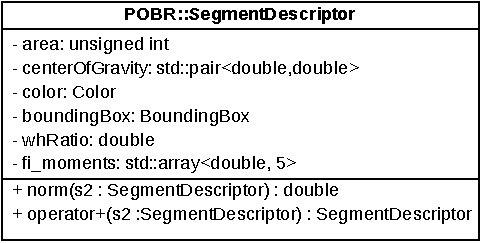
\includegraphics[width=\columnwidth]{figures/POBR-Class.pdf}
    \caption{Diagram UML klasy deskryptora segmentu}
    \label{fig:descriptor-uml}
\end{figure}

Razem z~deskryptorem, zdefiniowane zostały dwie operacje: dodawania segmentów oraz obliczania normy różnicy dwóch segmentów. Dodawanie segmentów polega na złączeniu dwóch list punktów oraz ponownym obliczeniu cech segmentów, natomiast obliczanie normy różnicy dwóch segmentów sprowadza się do policzenia sumy kwadratów różnic pomiędzy poszczególnymi momentami niezmienniczymi $\phi_{i}$, czyli odległości euklidesowskiej w~przestrzeni rozpiętej przez te momenty.

\subsubsection{Inne możliwe podejścia}
Przedstawiony powyżej sposób nie jest oczywiście jedynym możliwym. Inne podejście zakłada wykorzystanie deskryptorów tekstur. Żeby uzyskać liczbowy opis tekstury w~postaci wektora cech można posłużyć się:
\begin{itemize}
    \item metodami statystycznymi opartymi na histogramach kolorów, mierzącymi kontrast, granularność, gładkość i~chropowatość obszaru,
    \item metodami spektralnymi opartymi o~pomiary autokorelacji i~parametry obrazów przefiltrowanych częstotliwościowo,
    \item metodami strukturalnymi opartymi o~badanie struktury obszaru, kolor czy wektory ruchu~\cite{perm:wyklad}.
\end{itemize} 

Do badania tekstur można wykorzystać takie narzędzia jak macierz współwystępowania Haralicka czy filtry Gabora. 

Innym podejściem jest odrzucenie jawnych deskryptorów opisujących cechy obrazu i~zastosowanie uczenia maszynowego do automatycznego wykrywania cech. Najlepszym tego typu narzędziem jest splotowa sieć neuronowa. Każda warstwa splotowa przyjmuje na wejściu obraz lub mapę cech niższego poziomu i~tworzy nowy zbiór nowych map cech. Wyższe warstwy sieci splotowej agregują większe obszary obrazu. 

Uzyskane zbiory filtrów i~cech są optymalizowane względem konkretnego zestawu danych uczących, dlatego niekoniecznie muszą być łatwe w~ludzkiej iterpretacji~\cite{perm:wyklad}.